% concatenated from param_stoch_arxiv.tex
\documentclass{article}
\usepackage{fullpage}
\usepackage{amsthm}
\newtheorem{theorem}{Theorem}
\newtheorem{lemma}[theorem]{Lemma}
\newtheorem{proposition}[theorem]{Proposition}
\newenvironment{keywords}{\begin{center}Keywords:}{\end{center}}
\newcommand{\email}[1]{Email: #1}

\usepackage{amsmath,amssymb,amsfonts}
\usepackage{tikz}

\newcommand{\N}{\mathbb{N}}
\newcommand{\Z}{\mathbb{Z}}
\newcommand{\R}{\mathbb{R}}
\newcommand{\Q}{\mathbb{Q}}

\newcommand{\card}{\#}
\newcommand{\st}{\text{s.t.}}
\newcommand{\E}{\mathbb{E}}
\renewcommand{\P}{\mathbb{P}}
\newcommand{\B}{{\cal B}}
\newcommand{\NB}{{\cal N}}
\renewcommand{\d}{\,\textnormal{d}}
\newcommand{\medcup}{\scalebox{1.5}{$\cup$}}
\newcommand{\medcap}{\scalebox{1.5}{$\cap$}}
\DeclareMathOperator{\vol}{vol}
\newcommand{\e}{\mathbf{e}}

\title{A note on the complexity of two-stage stochastic linear optimization with small second stage}

\author{Christoph~Buchheim\thanks{Fakult\"at f\"ur Mathematik, TU Dortmund, Germany. \email{christoph.buchheim@tu-dortmund.de}}}

\begin{document}

\maketitle

\begin{abstract}
  Two-stage stochastic linear optimization is known to be \card P-hard
  when all involved random variables are independently and uniformly
  distributed over intervals, even with fixed recourse. We show that
  this problem is actually \card P-hard in the strong sense. More
  surprisingly, this hardness persists when the random vector is
  one-dimensional, i.e., uniformly distributed over a single
  interval. To obtain this result, we show that computing the area of
  a two-dimensional polytope given by a compact extended formulation
  is strongly \card P-hard.
  
  Furthermore, we obtain the same complexity result in case the number
  of second-stage constraints is fixed (for a problem in standard
  form), while fixing the number of second-stage variables leads to a
  weakly \card P-hard problem. Finally, if both the dimension of the
  random vector and the number of second-stage constraints are fixed,
  the problem turns out to be tractable.
\end{abstract}

\begin{keywords}
  Stochastic Optimization, \card P-hardness, Extended Formulations
\end{keywords}

\section{Introduction}

In two-stage stochastic optimization, some of the problem parameters
may depend on a random vector. The decision maker has to take some of
her decisions before the random variables are realized (the
\emph{first stage} or \emph{here-and-now} decisions), while the
remaining decisions can be taken afterwards (the \emph{second stage},
\emph{wait-and-see}, or \emph{recourse} decisions). The goal is to
optimize the expected objective value. The latter depends on the
probability distribution of the random parameters, which we assume to
be part of the input. In case of a linear optimization problem, the
two-stage stochastic counterpart can be stated as
\begin{equation}\label{prob:sslp}\tag{SSLP}
\begin{array}{rl}
  \min \quad & c^\top x +\E_\xi[Q(x,\xi)]\\[0.75ex]
  \st \quad & Ax\le b\;,
\end{array}
\end{equation}
where the second-stage objective value~$Q(x,\xi)$ depends on the
first-stage decision~$x$ and on a random variable~$\xi$, namely,
\begin{align*}
  Q(x,\xi) \; = \; \min \quad & q_\xi^\top y\\
  \st \quad & T_\xi x+W y=h_\xi,\quad y\ge 0\;.
\end{align*}
Here $c\in\R^{n_1}$, $A\in\R^{m_1\times n_1}$, and~$b\in\R^{m_1}$
describe the first-stage objective and constraints, where we assume
for the sake of simplicity that~$\{x\in\R^{n_1}\mid Ax\le b\}$ is
non-empty and bounded.  Moreover,~$q_\xi\in\R^{n_2}$,
$T_\xi\in\R^{m_2\times n_1}$, $W\in\R^{m_2\times n_2}$,
and~$h_\xi\in\R^{m_2}$ define the second-stage linear optimization
problem over the variables~$y\in\R^{n_2}$. We assume here
that~$q_\xi$, $T_\xi$, and $h_\xi$ depend on the random variable~$\xi$
in an affine-linear way. In this note, we restrict ourselves to the
case of fixed recourse, meaning that~$W$ does not depend on~$\xi$,
which is a common assumption in two-stage stochastic linear
optimization. For more details, we refer to the
textbook~\cite{Birge11}.

If the random variable~$\xi$ has finite support, it is easy to see
that~\eqref{prob:sslp} can be reformulated as an equivalent single
stage linear optimization problem. For this, we can essentially
introduce a copy of the second stage for each possible realization
of~$\xi$. In particular, problem~\eqref{prob:sslp} can be solved
efficiently if the support of~$\xi$ is given explicitly as part of the
input. This is not possible, however, if the distribution of~$\xi$ is
continuous or if the support is finite but exponential in the input.
In fact, the complexity picture changes drastically if~$\xi$ follows a
continuous uniform distribution, even if all entries of~$\xi$ are
independently distributed. In the remainder of this note, we
assume~$\xi\sim{\cal U}[l,u]$ with~$l,u\in\R^d$, $l<u$. It was shown
by Hanasusanto et al.\ \cite{Hanasusanto16} that~\eqref{prob:sslp} is
\card P-hard in this setting, even if only the objective
vector~$q_\xi$ is random. Since the objective in~\eqref{prob:sslp} is
convex in~$x$, the difficulty of solving~\eqref{prob:sslp} essentially
stems from the difficulty of computing objective values, i.e., of
computing~$\E_\xi[Q(x,\xi)]$ for a given first-stage
decision~$x$. This result even holds for~$n_1=1$, i.e., in case of a
single first-stage variable.

The proof presented in~\cite{Hanasusanto16} requires both an unbounded
number of second-stage variables and an unbounded dimension of the
random vector~$\xi$.  It is thus a natural question to ask which
complexity results persist if one or both of these parameters are
fixed. Surprisingly, to the best of our knowledge, these questions
have not been discussed in the literature so far -- although one could
argue that in practice the sample space is often low-dimensional, even
if many coefficients in the second-stage problem are affected by the
uncertainty. For instance, the only relevant random variables in an
agricultural application may be the amount of rain and sunshine during
a certain period. Moreover, using principle component analysis, the
dimension of the random vector can often be reduced without losing too
much in terms of solution quality. This motivated our investigation of
the complexity of~\eqref{prob:sslp} with fixed dimension~$d$.

Unfortunately, Problem~\eqref{prob:sslp} turns out to be \card P-hard
even when restricted to~$d=1$, i.e., to a single random variable
(Section~\ref{sec:fixed_d}), or to~$n_2=2$ and~$m_2=1$, i.e., to a
second-stage problem with very few variables and constraints
(Section~\ref{sec:fixed_mn}). Both is true even in the case of fixed
recourse and for~$n_1=1$. In fact, we show \card P-hardness in the
strong sense for~$d=1$ or~$m_2=1$. However, if both~$m_2$ and~$d$ are
fixed, the problem turns tractable (Section~\ref{sec:fixed_both}).

\section{Fixed dimension of the random vector}\label{sec:fixed_d}

We first discuss the special case of Problem~\eqref{prob:sslp} where
the dimension~$d$ of the random vector is fixed. Our aim is to reduce
\card IS, the \card P-complete counting version of the independent set
problem, to the restriction of~\eqref{prob:sslp} with~$d=1$. This will
imply that the latter restriction is still \card P-hard, even in the
strong sense. To this end, we use a construction that is inspired by
the extended formulation of a regular polygon presented by Ben-Tal and
Nemirovski~\cite{BenTal01}. For the following, let~$Q_k$ denote the
regular $k$-gon centered in the origin with vertices
\[
v_i:=\sec(\tfrac\pi k)(\cos((2i+1)\tfrac\pi k),\sin((2i+1)\tfrac\pi
k))^\top,\quad i=0,\dots,k-1\;.\] Then $||v_i||=\sec(\tfrac\pi k)$ for
all~$i=0,\dots,k-1$ and~$\vol(Q_{k})=k\tan(\tfrac\pi k)$.  The center
point of the facet of~$Q_k$ connecting~$v_i$ and~$v_{i+1}$
(setting~$v_{k}:=v_0$) is denoted by
\[
w_i:=\tfrac 12(v_i+v_{i+1})=(\cos((2i+2)\tfrac\pi
k),\sin((2i+2)\tfrac\pi k))^\top\;,\] it has length~$||w_i||=1$ and
agrees with the normal vector of the corresponding facet for
all~$i=0,\dots,k-1$.

Now to start the construction, let a simple undirected graph~$G=(V,E)$
be given, where we assume $V=\{1,\dots,n\}$ with~$n\ge 2$. Consider
the polyhedron
\begin{eqnarray*}
  P^\emptyset_n ~ := ~ & \big\{ & (y,z)\in\R^{n+1}\times\R^{n+1}\mid\\
  && \; \left.\begin{array}{l}
    \; y_{i+1} = \cos(\tfrac\pi{2^{i-1}})y_{i}+\sin(\tfrac\pi{2^{i-1}})z_{i}\\[1ex]
    \; z_{i+1} \ge -\sin(\tfrac\pi{2^{i-1}})y_{i}+\cos(\tfrac\pi{2^{i-1}})z_{i}\\[1ex]
    \; z_{i+1} \ge +\sin(\tfrac\pi{2^{i-1}})y_{i}-\cos(\tfrac\pi{2^{i-1}})z_{i}
  \end{array} ~ \right\} ~ \forall i=1,\dots,n\\
  &&\quad\;  y_{n+1} \le 1, ~ \cos(\tfrac\pi{2^{n-1}})y_{n+1}+\sin(\tfrac\pi{2^{n-1}})z_{n+1}\le 1\big\}\;.
\end{eqnarray*}
This formulation contains the matrix
\[
R_i:=\begin{pmatrix} \cos(\tfrac\pi{2^{i-1}}) &
\sin(\tfrac\pi{2^{i-1}})\\ -\sin(\tfrac\pi{2^{i-1}}) &
\cos(\tfrac\pi{2^{i-1}})\\
\end{pmatrix}
\]
which describes the clockwise rotation in~$\R^2$ around the origin
by~$\tfrac\pi{2^{i-1}}$ degrees, i.e., by one $2^i$-th of a full
rotation. Moreover, we will denote by~$R$ the reflection in~$\R^2$
with respect to the first axis, which flips the sign of the second
entry. The geometric idea behind the construction in~\cite{BenTal01}
is captured in the following lemma.

\begin{lemma}\label{lem:basic}
  For each vertex~$v_\ell$ of~$Q_{2^n}$, there exists a
  unique~$b^\ell\in\{0,1\}^n$ with
  \[
  R^{b^\ell_n}R_n\cdots R^{b^\ell_1}R_1 v_\ell=v_0\;.
  \]
\end{lemma}
\begin{proof}
  To show existence, we define~$b^\ell$ recursively for~$i=1,\dots,n$,
  setting~$b^\ell_i:=1$ if and only
  if
  $$R_{i}R^{b^\ell_{i-1}}R_{i-1}\cdots R^{b^\ell_1}R_1 v_\ell$$
  has a
  negative second entry. Then it follows by induction that the angle
  of~$R^{b^\ell_{i}}R_{i}\cdots R^{b^\ell_1}R_1 v_\ell$ lies in the
  range~$[0,\tfrac\pi{2^{i-1}}]$. In particular, the final
  vector~$v=R^{b^\ell_{n}}R_{n}\cdots R^{b^\ell_1}R_1 v_\ell$ has an
  angle in~$[0,\tfrac\pi{2^{n-1}}]$. Moreover,~$v=v_{\ell'}$ for
  some~$\ell'\in\{0,\dots,2^n-1\}$, since all involved rotations and
  reflections permute the vertices of~$Q_{2^n}$. Thus~$v=v_0$, the
  only vertex with angle in~$[0,\tfrac\pi{2^{n-1}}]$.

  To show uniqueness, let~$b\in\{0,1\}^n\setminus\{b^\ell\}$ and
  let~$i$ be minimal with~$b_i\neq b^\ell_i$. Then~$R^{b_i}R_{i}\cdots
  R^{b_1}R_1 v_\ell$ has a non-positive second entry and an angle
  in~$[\tfrac\pi{2^{i-1}},2\pi]$. It follows by induction
  that~$R^{b_j}R_{j}\cdots R^{b_1}R_1 v_\ell$ has an angle
  in~$[\tfrac\pi{2^{j-1}},2\pi]$ for all~$j\ge i$,
  hence~$R^{b_n}R_{n}\cdots R^{b_1}R_1 v_\ell$ cannot agree
  with~$v_0$, which has an angle of~$\tfrac\pi{2^n}$.
\end{proof}
By Lemma~\ref{lem:basic}, the vertices~$v_\ell$ of~$Q_{2^n}$ are in
one-to-one correspondence with the binary
vectors~$b_\ell\in\{0,1\}^n$; see Figure~\ref{fig:vertices} for an
illustration. In particular, they correspond to the subsets of~$V$
via~$S_\ell:=\{i\in V\mid b^\ell_i=0\}$. Note that the connection
between~$\ell$ and~$b^\ell$ is different from the standard binary
expansion of~$\ell$.
\begin{figure}
  \begin{center}
    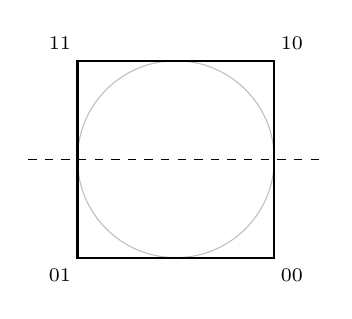
\begin{tikzpicture}[scale=1.25]
      \def\k{4}
      \foreach \i in {1,...,\k} {
        \pgfmathsetmacro{\angle}{(2*\i-1)*180/\k}
        \pgfmathsetmacro{\radius}{1/cos(180/\k)}
        \coordinate (v\i) at ({\radius*cos(\angle)}, {\radius*sin(\angle)});
      }
      \draw[thin,gray!50!white] (0,0) circle (1);
      \draw[thick] (v1) \foreach \i in {2,...,\k} { -- (v\i) } -- cycle;
      \foreach \i in {1,...,\k} {
        \pgfmathsetmacro{\angle}{(2*\i-1)*180/\k}
        \ifcase\i
        \or
        \def\label{10}
        \or
        \def\label{11}
        \or
        \def\label{01}
        \or
        \def\label{00}
        \fi
        \def\slabel{\scriptsize{\label}};
        \node[shift={(\angle:9pt)}] at (v\i) {\slabel};
      }
      \draw[dashed] (-1.5,0)--(1.5,0);
    \end{tikzpicture}
    \qquad
    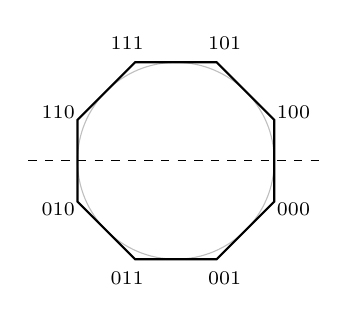
\begin{tikzpicture}[scale=1.25]
      \def\k{8}
      \foreach \i in {1,...,\k} {
        \pgfmathsetmacro{\angle}{(2*\i-1)*180/\k}
        \pgfmathsetmacro{\radius}{1/cos(180/\k)}
        \coordinate (v\i) at ({\radius*cos(\angle)}, {\radius*sin(\angle)});
      }
      \draw[thin,gray!50!white] (0,0) circle (1);
      \draw[thick] (v1) \foreach \i in {2,...,\k} { -- (v\i) } -- cycle;
      \foreach \i in {1,...,\k} {
        \pgfmathsetmacro{\angle}{(2*\i-1)*180/\k}
        \ifcase\i
        \or
        \def\label{100}
        \or
        \def\label{101}
        \or
        \def\label{111}
        \or
        \def\label{110}
        \or
        \def\label{010}
        \or
        \def\label{011}
        \or
        \def\label{001}
        \or
        \def\label{000}
        \fi
        \def\slabel{\scriptsize{\label}};
        \node[shift={(\angle:7.5pt)}] at (v\i) {\slabel};
      }
      \draw[dashed] (-1.5,0)--(1.5,0);
    \end{tikzpicture}
  \end{center}
  \caption{The regular $2^n$-gon $Q_{2^n}$ for $n=2,3$ and the binary
    vectors~$b^\ell$ assigned to its vertices.}\label{fig:vertices}
\end{figure}
We also remark that~$R^{b^\ell_n}R_n\cdots R^{b^\ell_1}R_1$ maps any
vector with an angle in~$[\ell\tfrac \pi{2^{n-1}},(\ell+1)\tfrac
  \pi{2^{n-1}}]$, i.e., between the angles of~$w_{\ell-1}$
and~$w_\ell$, to a vector with angle in~$[0,\tfrac \pi{2^{n-1}}]$.

The following result is shown in~\cite[Prop.~2.1]{BenTal01}, but we
give a slightly different proof here, as its core idea is essential
for motivating the rest of the construction.
\begin{proposition}\label{prop:proj}
  The projection $\bar P^\emptyset_n$ of~$P^\emptyset_n$
  to~$(y_1,z_1)$ agrees with~$Q_{2^n}$.
\end{proposition}
\begin{proof}
  To show~$Q_{2^n}\subseteq \bar P^\emptyset_n$, it suffices to
  consider the vertices~$v_\ell$ of~$Q_{2^n}$. Then
  defining~$(y_1,z_1)^\top:=v_\ell$
  and~$(y_{i+1},z_{i+1})^\top:=R^{b^\ell_i}R_i(y_i,z_i)^\top$,
  for~$i=1,\dots,n$, yields a vector~$(y,z)$ that satisfies the
  recursive constraints in~$P^\emptyset_n$ by
  construction. Furthermore, we obtain
  $(y_{n+1},z_{n+1})^\top=v_0=(1,\tan(\tfrac\pi{2^n}))^\top$ from
  Lemma~\ref{lem:basic}, which satisfies the remaining two
  constraints.

  For the other inclusion, let~$(y,z)\in P^\emptyset_n$. We show
  that~$(y_1,z_1)$ then satisfies all facet-defining inequalities
  for~$Q_{2^n}$, i.e.,~$w_\ell^\top (y_1,z_1)^\top\le 1$ for
  each~$\ell$.  As mentioned above, $R^{b^\ell_i}R_i\cdots
  R^{b^\ell_1}R_1w_\ell$ has a non-negative second entry for
  all~$i=1,\dots,n$. In particular, since all involved rotations and
  reflections are orthogonal, we obtain
  \begin{eqnarray*}
    w_\ell^\top(y_1,z_1)^\top
    & = & (R^{b^\ell_1}R_1w_\ell)^\top R^{b^\ell_1}R_1(y_1,z_1)^\top\\
    & \le & (R^{b^\ell_1}R_1w_\ell)^\top (y_2,z_2)^\top\\
    & = & (R^{b^\ell_2}R_2R^{b^\ell_1}R_1w_\ell)^\top R^{b^\ell_2}R_2(y_2,z_2)^\top\\
    & \le & (R^{b^\ell_2}R_2R^{b^\ell_1}R_1w_\ell)^\top (y_3,z_3)^\top\\
    & \vdots & \\
    & \le & (R^{b^\ell_n}R_n\cdots R^{b^\ell_1}R_1w_\ell)^\top (y_{n+1},z_{n+1})^\top\\
    & = & w_0^\top (y_{n+1},z_{n+1})^\top\\
    & = & \cos(\tfrac\pi{2^{n-1}})y_{n+1}+\sin(\tfrac\pi{2^{n-1}})z_{n+1}\le 1\;,
  \end{eqnarray*}
  which yields the desired result.
\end{proof}
In the recursive construction of~$(y,z)$ from~$v_\ell$ described
above, the vector~$R_i(y_{i},z_{i})^\top$ is reflected if and only
if~$b^\ell_i=1$. We will exploit this for cutting off from~$\bar
P_n^\emptyset$ exactly those vertices corresponding to dependent sets
in~$G$. To this end, we define a further polyhedron for each
edge~$e\in E$ as follows:
\begin{eqnarray*}
  P^e_n:= & \big\{ & (y,z)\in\R^{n+1}\times\R^{n+1}\mid\\
  && \left.\begin{array}{l}
    \,\,y_{i+1} = \cos(\tfrac\pi{2^{i-1}})y_{i}+\sin(\tfrac\pi{2^{i-1}})z_{i}\\[1ex]
    \,\,z_{i+1} = -\sin(\tfrac\pi{2^{i-1}})y_{i}+\cos(\tfrac\pi{2^{i-1}})z_{i} \hspace*{4.25ex} \text{ if~$i\in e$}\\[1ex]
    \hspace*{-0.66ex}\left.\begin{array}{l}
    z_{i+1} \ge -\sin(\tfrac\pi{2^{i-1}})y_{i}+\cos(\tfrac\pi{2^{i-1}})z_{i}\\[1ex]
    z_{i+1} \ge +\sin(\tfrac\pi{2^{i-1}})y_{i}-\cos(\tfrac\pi{2^{i-1}})z_{i}
    \end{array}
    ~ \right\} \text{ if~$i\not\in e$}
  \end{array}\right\} ~ \forall i=1,\dots,n\\
  &&\;\;\;\, \cos(\tfrac\pi{2^n})y_{n+1}+\sin(\tfrac\pi{2^n})z_{n+1}\le \cos(\tfrac\pi{2^n})
  \big\}
\end{eqnarray*}
Finally, we denote by~$\bar P^e_n$ the projection of~$P^e_n$
to~$(y_1,z_1)$ and define
\[
\bar P_G:=\underset{e\in E\cup\{\emptyset\}}{\medcap}\bar P^e_n\;.
\]
In summary, we have constructed an extended formulation of the
two-dimensional polytope~$\bar P_G$ that can be computed in polynomial
time from the graph~$G$. We will show that we can derive the number of
independent sets of~$G$ from the area of~$\bar P_G$.
\begin{lemma}\label{lem:main}
  For each~$e\in E$, the intersection $\bar
  P^\emptyset_n\cap\bar P^e_n$ agrees with the closure of
  \[
  Q_{2^n}\setminus\underset{\ell:\,e\subseteq
    S_\ell}{\medcup}\Delta_\ell\;,
  \]
  where $\Delta_\ell$ is the triangle spanned by~$w_{\ell-1}$,
  $v_\ell$, and~$w_{\ell}$.
\end{lemma}
\begin{proof}
  It suffices to show the following three statements:
  \begin{itemize}
  \item[(a)] $w_\ell\in\bar P^e_n$ for all~$\ell=0,\dots,2^n-1$.
  \item[(b)] If~$e\not\subseteq S_\ell$, then $v_\ell\in \bar P^e_n$.
  \item[(c)] If~$e\subseteq S_\ell$, the maximum of~$v_\ell^\top
    (y_1,z_1)^\top$ over~$\bar P_n^e$ is attained at~$w_{\ell-1}$
    and~$w_{\ell}$.
  \end{itemize}
  For (a), we again define~$(y,z)\in P_n^e$ recursively. Starting
  with~$(y_1,z_1)^\top:=w_\ell$, we set
  $(y_{i+1},z_{i+1})^\top:=R_i(y_i,z_i)^\top$ if~$i\in e$ or if the
  second entry of~$R_i(y_i,z_i)^\top$ is non-negative,
  and~$(y_{i+1},z_{i+1})^\top:=RR_i(y_i,z_i)^\top$ otherwise. Then the
  resulting vector~$(y,z)$ satisfies all recursive constraints
  and~$(y_{n+1},z_{n+1})$ agrees with~$w_{\ell'}$ for
  some~$\ell'\in\{0,\dots,2^n-1\}$, thus it also satisfies the last
  constraint in~$P_n^e$.

  For (b), we use the same construction as in (a), now starting
  with~$(y_1,z_1)^\top=v_\ell$. Since~$e\not\subseteq S_\ell$, we must
  obtain~$(y_{n+1},z_{n+1})^\top=R^{b_n}R_n\cdots R^{b_1}R_1v_\ell$
  with~$b\neq b^\ell$, so that~$(y_{n+1},z_{n+1})^\top=v_{\ell'}$
  with~$\ell'\neq 0$. It follows again that~$(y_{n+1},z_{n+1})$
  satisfies the last constraint in~$P_n^e$.

  Finally, to show (c), let~$e\subseteq S_\ell$. Then we
  obtain~$v_\ell^\top(y_1,z_1)\le v_0^\top(y_{n+1},z_{n+1})$ exactly
  as in the second direction of the proof of
  Proposition~\ref{prop:proj}, except that the $i$-th and $j$-th
  inequalities now turn into equations for~$e=\{i,j\}$. From the last
  constraint, we thus derive~$v_\ell^\top(y_1,z_1)\le 1$, and this
  bound is attained at~$w_{\ell-1}$ and~$w_\ell$.
\end{proof}
\noindent The statement of Lemma~\ref{lem:main} is illustrated in
Figure~\ref{fig:main}.
\begin{figure}
  \begin{center}
    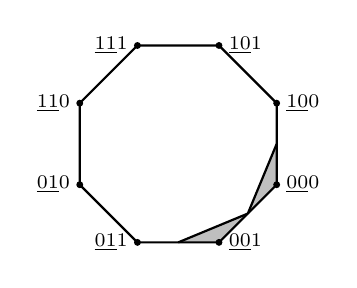
\begin{tikzpicture}[scale=1.25]
      \def\k{8}
      \foreach \i in {1,...,\k} {
        \pgfmathsetmacro{\angle}{(2*\i-1)*180/\k}
        \pgfmathsetmacro{\radius}{1/cos(180/\k)}
        \coordinate (v\i) at ({\radius*cos(\angle)}, {\radius*sin(\angle)});
        \coordinate (w\i) at ({cos(\angle+180/\k)}, {sin(\angle+180/\k)});
      }

      \fill[gray!50] (v7) -- (w7) -- (w6) -- cycle;
      \draw[thick] (w7) -- (w6);
      \fill[gray!50] (v8) -- (w8) -- (w7) -- cycle;
      \draw[thick] (w8) -- (w7);

      \draw[thick] (v1) \foreach \i in {2,...,\k} { -- (v\i) } -- cycle;
      \foreach \i in {1,...,\k} {
        \fill (v\i) circle (1pt);
      }

      \draw (v1) node[right]{\scriptsize \underline{10}0};
      \draw (v2) node[right]{\scriptsize \underline{10}1};
      \draw (v3) node[left]{\scriptsize \underline{11}1};
      \draw (v4) node[left]{\scriptsize \underline{11}0};
      \draw (v5) node[left]{\scriptsize \underline{01}0};
      \draw (v6) node[left]{\scriptsize \underline{01}1};
      \draw (v7) node[right]{\scriptsize \underline{00}1};
      \draw (v8) node[right]{\scriptsize \underline{00}0};

    \end{tikzpicture}
    \quad
    \begin{tikzpicture}[scale=1.25]
      \def\k{8}
      \foreach \i in {1,...,\k} {
        \pgfmathsetmacro{\angle}{(2*\i-1)*180/\k}
        \pgfmathsetmacro{\radius}{1/cos(180/\k)}
        \coordinate (v\i) at ({\radius*cos(\angle)}, {\radius*sin(\angle)});
      }

      \fill[gray!50] (v5) -- (w5) -- (w4) -- cycle;
      \draw[thick] (w5) -- (w4);
      \fill[gray!50] (v8) -- (w8) -- (w7) -- cycle;
      \draw[thick] (w8) -- (w7);

      \draw[thick] (v1) \foreach \i in {2,...,\k} { -- (v\i) } -- cycle;
      \foreach \i in {1,...,\k} {
        \fill (v\i) circle (1pt);
      }

      \draw (v1) node[right]{\scriptsize \underline{1}0\underline{0}};
      \draw (v2) node[right]{\scriptsize \underline{1}0\underline{1}};
      \draw (v3) node[left]{\scriptsize \underline{1}1\underline{1}};
      \draw (v4) node[left]{\scriptsize \underline{1}1\underline{0}};
      \draw (v5) node[left]{\scriptsize \underline{0}1\underline{0}};
      \draw (v6) node[left]{\scriptsize \underline{0}1\underline{1}};
      \draw (v7) node[right]{\scriptsize \underline{0}0\underline{1}};
      \draw (v8) node[right]{\scriptsize \underline{0}0\underline{0}};
    \end{tikzpicture}
    \quad
    \begin{tikzpicture}[scale=1.25]
      \def\k{8}
      \foreach \i in {1,...,\k} {
        \pgfmathsetmacro{\angle}{(2*\i-1)*180/\k}
        \pgfmathsetmacro{\radius}{1/cos(180/\k)}
        \coordinate (v\i) at ({\radius*cos(\angle)}, {\radius*sin(\angle)});
      }

      \fill[gray!50] (v5) -- (w5) -- (w4) -- cycle;
      \draw[thick] (w5) -- (w4);
      \fill[gray!50] (v7) -- (w7) -- (w6) -- cycle;
      \draw[thick] (w7) -- (w6);
      \fill[gray!50] (v8) -- (w8) -- (w7) -- cycle;
      \draw[thick] (w8) -- (w7);

      \draw[thick] (v1) \foreach \i in {2,...,\k} { -- (v\i) } -- cycle;
      \foreach \i in {1,...,\k} {
        \fill (v\i) circle (1pt);
      }
      \draw (v1) node[right]{\scriptsize 100};
      \draw (v2) node[right]{\scriptsize 101};
      \draw (v3) node[left]{\scriptsize 111};
      \draw (v4) node[left]{\scriptsize 110};
      \draw (v5) node[left]{\scriptsize 010};
      \draw (v6) node[left]{\scriptsize 011};
      \draw (v7) node[right]{\scriptsize 001};
      \draw (v8) node[right]{\scriptsize 000};
    \end{tikzpicture}
  \end{center}
  \caption{Illustration of Lemma~\ref{lem:main} for~$V=\{1,2,3\}$
    and $E=\{\{1,2\},\{1,3\}\}$. From left to right, the
    polygons~$\bar P_n^\emptyset\cap\bar P_n^{\{1,2\}}$, $\bar
    P_n^\emptyset\cap\bar P_n^{\{1,3\}}$, and $\bar P_G$ are depicted,
    where the shaded areas mark the triangles~$\Delta_\ell$ not
    belonging to the respective polygon. In~$\bar P_G$, the latter
    triangles correspond to the three dependent sets~$\{1,2\}$,
    $\{1,3\}$, and~$\{1,2,3\}$ in~$G$.}\label{fig:main}
\end{figure}
It is now easy to derive
\begin{theorem}\label{theo:vol}
  It is strongly \card P-hard to compute $\vol(\bar P_G)$ up to an
  additive error of less than
  $$\tfrac 14\tan(\tfrac\pi{2^n})(1-\cos(\tfrac\pi{2^{n-1}}))\;.$$
\end{theorem}
\begin{proof}
  The interiors of all triangles~$\Delta_\ell$ are pairwise disjoint
  and have the same area $\delta:=\tfrac
  12\tan(\tfrac\pi{2^n})(1-\cos(\tfrac\pi{2^{n-1}}))$. Moreover, by
  Lemma~\ref{lem:main}, the triangle $\Delta_\ell$ is missing
  in~$\bar P_G$ if and only if there exists an edge~$e$
  with~$e\subseteq S_\ell$, i.e., if and only if~$S_\ell$ is a
  dependent set in~$G$. We derive that $\vol(\bar
  P_G)=\vol(Q_{2^{n}})-(2^n-n_{\text{IS}})\delta$, where
  $n_{\text{IS}}$ is the number of independent sets in~$G$. Hence
  \[
  n_{\text{IS}}=2^n-\tfrac 1\delta(\vol(Q_{2^n})-\vol(\bar P_G))
  \]
  can be computed efficiently from $\vol(\bar P_G)$ if the latter is
  known up to an additive error of less than~$\tfrac
  12\delta$. However, it is strongly \card P-complete to
  compute~$n_{\text{IS}}$, even on graphs with maximal degree
  three~\cite[Theorem~4.2]{Dyer00}.
\end{proof}
\begin{lemma}\label{lem:prec}
  For~$n\ge 2$, we have $\delta>\tfrac 1{2^{3n-3}}$.
\end{lemma}
\begin{proof}
  Since~$\tfrac\pi{2^{n-1}}\in [0,\tfrac\pi 2]$, we
  obtain~$\tan(\tfrac\pi{2^n})\ge\tfrac 1{2^{n-1}}$
  and~$1-\cos(\tfrac\pi{2^{n-1}})> \tfrac 1{2^{2n-3}}$ and thus the
  desired lower bound.
\end{proof}
\begin{theorem}\label{theo:small_d}
  Problem~\eqref{prob:sslp} is strongly \card P-hard for~$d=1$
  and~$n_1=1$, even if only the right hand side~$h_yi$ is random.
\end{theorem}
\begin{proof}
  Since~$\bar P_G$ is convex and contains both~$(-1,0)$ and~$(1,0)$,
  we have
  \begin{eqnarray*}
    \vol(\bar P_G)
    & = & \textstyle \int_{-1}^1 (\max\{z_1\mid (y_1,z_1)\in \bar P_G\}-\min\{z_1\mid (y_1,z_1)\in \bar P_G\}) \d y_1\\
    & = & 2\E_\xi[\max\{z_1\mid (\xi,z_1)\in \bar P_G\}]-2\E_\xi[\min\{z_1\mid (\xi,z_1)\in \bar P_G\}]
  \end{eqnarray*}
  with~$\xi\sim{\cal U}[-1,1]$. In view of Theorem~\ref{theo:vol}, it
  remains to show that the computation of $\E_\xi[\max\{z_1\mid
    (\xi,z_1)\in \bar P_G\}]$ can be polynomially reduced
  to~\eqref{prob:sslp} with~$n_1=1$; the min-case is analogous.  For
  this, similar to~\cite{Hanasusanto16}, we consider the problem of
  minimizing
  \[
  -cx+\E_\xi[\max\{z_1\mid (\xi,z_1)\in x\bar
    P_G\}]=x(\E_\xi[\max\{z_1\mid (\xi,z_1)\in \bar P_G\}]-c)
  \]
  over
  the single first-stage variable~$x\in [0,1]$. This is a problem of
  type~\eqref{prob:sslp}. Indeed, an extended formulation of~$x\bar
  P_G$ is obtained by multiplying all right-hand sides
  in~$P_n^\emptyset$ and in all $P_n^e$ with~$x$, so that the former
  right hand side now takes the role of the matrix~$T$, which is
  fixed. Moreover, the former variable~$y_1$, now replaced by~$\xi$,
  moves to the right hand side.
  
  If the optimum is attained at~$x=0$, we derive~$\E_\xi[\max\{z_1\mid
    (\xi,z_1)\in \bar P_G\}]\ge c$, otherwise~$\E_\xi[\max\{z_1\mid
    (\xi,z_1)\in \bar P_G\}]\le c$. Using a standard bisection
  approach for~$c$ in the range~$[\tfrac 12,1]$, the computation of
  the value~$\E_\xi[\max\{z_1\mid (\xi,z_1)\in \bar P_G\}]$ can thus
  be reduced to at most~$3n-3$ calls to~\eqref{prob:sslp} by
  Lemma~\ref{lem:prec}.
\end{proof}
The statement of Theorem~\ref{theo:small_d} also holds if, instead of
the right hand side~$h_\xi$, only the objective~$q_\xi$ is random. For
this, it suffices to dualize the given extended formulation
of~$(\xi,z_1)\in \bar P_G$ and scale by~$x$ afterwards.

\section{Fixed size of the second-stage problem}\label{sec:fixed_mn}

We next prove that bounding the number of variables and constraints in
the second stage is not sufficient to obtain a tractable special
case of~\eqref{prob:sslp} either. This can be shown by similar techniques as
employed in~\cite{Hanasusanto16}, although in the reduction presented
there, the second stage is not bounded and only weak \card P-hardness
is shown for the case of fixed recourse. We first fix only the number
of constraints~$m_2$.
\begin{theorem}\label{theo:small_m2}
  Problem~\eqref{prob:sslp} is strongly \card P-hard if~$n_1=1$
  and~$m_2=1$, even if only the objective~$q_\xi$ is random.
\end{theorem}
\begin{proof}
  Let~$P=\{\xi\in [0,1]^d\mid A\xi\le b\}$ be any non-empty polytope
  with~$A\in\Z^{m\times d}$ and~$b\in\Z^m$, for any~$m\in\N$. Then
  computing the volume of~$P$ is strongly \card
  P-hard~\cite{Dyer88}. For~$x\in[0,1]$ and~$t\in\R$, we consider the
  following second-stage problem
  \begin{align*}
    Q_{t}(x,\xi) \; = \; \max \quad & (A\xi-b-te)^\top y\\
    \st \quad & y\ge 0,\quad e^\top y\le x\;,
  \end{align*}
  where~$e=(1,\dots,1)^\top\in\R^m$. Transformed into standard form,
  we thus have~$m_2=1$ and~$n_2=m+1$.  Then
  \[
  Q_{t}(x,\xi)=\max\,\{0,\max\,\{a_j \xi-b_j\mid j=1,\dots,m\}-t\}\cdot x\;,
  \]
  where~$a_j$ denotes the $j$th row vector of~$A$, and
  \[
  \tfrac\partial{\partial t} Q_{t}(x,\xi)=\left\{\begin{array}{cl}
  0 & \text{if }A\xi< b+te \\
  -x & \text{if }a_j\xi > b_j+t\text{ for some }j\in\{1,\dots,m\}
  \end{array}\right.
  \]
  Hence, using the Leibniz integral rule and assuming~$\xi\sim{\cal
    U}[0,1]^d$,
  \[
  \tfrac\partial{\partial t} \E_\xi[Q_{t}(x,\xi)]
  = \E_\xi[\tfrac\partial{\partial t} Q_{t}(x,\xi)]
  = (\vol(P_t)-1)\cdot x\;,
  \]
  where~$P_t=\{\xi\in [0,1]^d\mid A\xi\le b+te\}$. Now
  define~$p(t):=\E_\xi[Q_t(x,\xi)]$. By Lemma~\ref{lem:polynomial} in
  Appendix~\ref{app}, the derivative~$p'(t)=(\vol(P_t)-1)x$ is a
  polynomial of degree at most~$d$ in the range~$[0,1]$. Hence~$p$ is a
  polynomial of degree at most~$d+1$ in the same range, and the~$d+2$
  coefficients of~$p$ can be obtained by evaluating~$p$ at~$d+2$
  different points in~$[0,1]$; the derivative~$p'$ can then be
  determined symbolically.  Altogether, for~$x>0$, the computation
  of~$\vol(P)$ can be polynomially reduced to the computation
  of~$\E_\xi[Q_{t}(x,\xi)]$ for different values of~$t\in\R$, so that
  the latter task is strongly \card P-hard. Arguing analogously to the
  last part of the proof of Theorem~\ref{theo:small_d}, it follows
  that~\eqref{prob:sslp} is strongly \card P-hard for~$n_1=m_2=1$.
\end{proof}
If the polytope~$P$ in the proof of Theorem~\ref{theo:small_m2} is
defined by only one linear inequality, it is still (weakly) \card
P-hard to compute the volume of~$P$~\cite{Dyer88}. We thus obtain
\begin{theorem}\label{theo:small_n2}
  Problem~\eqref{prob:sslp} is \card P-hard if~$n_1=1$,~$n_2=2$,
  and~$m_2=1$, even if only the objective~$q_\xi$ is random.
\end{theorem}

Comparing the results of Theorem~\ref{theo:small_m2} and
Theorem~\ref{theo:small_n2}, it remains to clarify whether
fixing~$n_2$ (and thus also~$m_2$) leads to a strongly or weakly \card
P-hard problem. The latter is the case.
\begin{theorem}\label{theo:pseudo}
  Let~$n_2$ be fixed. Then~\eqref{prob:sslp} can be solved up to any
  desired accuracy~$\varepsilon>0$ in pseudopolynomial time (and in
  time logarithmic in~$1/\varepsilon$).
\end{theorem}
\begin{proof}
  It is easy to verify that $\E_\xi[Q(x,\xi)]$ is a convex function
  in~$x$, thus by Grötschel et al.~\cite[Theorem~4.3.13]{Grotschel93}
  -- and due to our assumption that the first-stage feasible region is
  non-empty and bounded -- it suffices to show that~$\E_\xi[Q(x,\xi)]$
  can be computed in pseudopolynomial time for any given~$x\in\R^n$.

  Let~$B$ be the set of bases of~$W$. Since~$n_2$ is fixed and~$m_2\le
  n_2$, also~$|B|\le n_2^{m_2}$ is bounded. For each~$\B\in B$,
  let~$P_\B$ denote the set of all~$\xi\in[l,u]^d$ such that~$\B$ is
  feasible and optimal for the given~$x$, i.e.,
  \[
  P_\B:=\{\xi\in [l,u]^d\mid W_\B^{-1}(h_\xi-T_\xi x)\ge
  0,~(q_\xi)_\NB-W_\NB^\top (W_\B^{-1})^\top(q_\xi)_\B\ge 0\}\;.
  \]
  Each~$P_\B$ is a polytope defined by intersecting
  the box~$[l,u]^d$ with~$n_2$ many halfspaces.
  
  Next, we partition~$B$ into equivalence
  classes~$B^{(1)},\dots,B^{(\ell)}$ with respect to the quadratic
  function $(q_\xi)_{\B}^\top W_{\B}^{-1}(h_\xi-T_\xi x)$ that
  describes the objective value of the basic solution corresponding
  to~$\B$ as a function of~$\xi$. More precisely, two bases are
  equivalent if this function agrees on~$\R^d$; we denote the latter
  by~$q^{(r)}$ for the class~$B^{(r)}$. Two bases~$\B_1$ and~$\B_2$
  belonging to different classes are simultaneously optimal on a zero
  set, so that~$\vol(P_{\B_1}\cap P_{\B_2})=0$. In particular,
  setting~$P^{(r)}:=\cup_{\B\in B^{(r)}}P_{\B}$, we obtain
  \[
  \E_\xi[Q(x,\xi)] = \E_\xi\big[\max_{\B\in B}\;(q_\xi)_\B^\top W_\B^{-1}(h_\xi-T_\xi x)\big]
  = \Big(\prod_{i=1}^d\tfrac 1{u_i-l_i}\Big)\sum_{r=1}^\ell \int_{P^{(r)}} q^{(r)}(\xi) \d\xi\;.
  \]
  By the inclusion-exclusion principle, we have
  \begin{equation}
    \int_{P^{(r)}} q^{(r)}(\xi) \d\xi
    = \sum_{\emptyset\neq B'\subseteq B^{(r)}}(-1)^{|B'|+1}
    \int_{\cap_{\B\in B'} P_{\B}} q^{(r)}(\xi)\d\xi\;.\label{eq:incl_excl}\tag{*}
  \end{equation}\\[-1.5ex]
  Since~$|B^{(r)}|\le |B|\le n_2^{m_2}$, this sum ranges over at
  most~$2^{n_2^{m_2}}-1$ many subsets and each
  intersection~$\cap_{\B\in B'} P_{\B}$ is a polytope defined by box
  constraints and at most~$n_2^{m_2+1}$ linear inequalities. All
  integrals in~\eqref{eq:incl_excl} can thus be computed in
  pseudopolynomial time by Lemma~\ref{lem:quad} in
  Appendix~\ref{app}. This yields the desired result.
\end{proof}

\section{Fixing both sizes}\label{sec:fixed_both}

We finally discuss the case where both the dimension~$d$ of the random
vector and the number~$m_2$ of second-stage constraints are fixed.
\begin{theorem}\label{theo:both}
  Let~$d$ and~$m_2$ be fixed. Then~\eqref{prob:sslp} can be solved up
  to any desired accuracy~$\varepsilon>0$ in polynomial time (and in
  time logarithmic in~$1/\varepsilon$).
\end{theorem}
\begin{proof}
  The result can be shown analogously to
  Theorem~\ref{theo:pseudo}. Again, it suffices to
  compute~$\E_\xi[Q(x,\xi)]$, but the number of second-stage
  bases~$|B|$ is now polynomial instead of fixed. In particular, the
  number of non-zero terms in the sum in~\eqref{eq:incl_excl} can now
  become exponential. However, the total number of constraints
  defining all polytopes~$P_{\cal B}$ with~${\cal B}\in B^{(r)}$
  is~$n_2^{m_2+1}$ and hence polynomial, as~$m_2$ is fixed. Since~$d$
  is fixed as well, we can compute the corresponding hyperplane
  arrangement and identify all cells belonging to~$P^{(r)}$ in
  polynomial time; see, e.g.,~\cite{Edelsbrunner86}. Finally,
  integrating~$q^{(r)}$ over~$P^{(r)}$ reduces to
  integrating~$q^{(r)}$ over these cells, which can be done
  efficiently for fixed~$d$ using triangulation; see,
  e.g.,~\cite{Lawrence91}.
\end{proof}

\section{Conclusion}

The following table summarizes all results. Recall that~$m_2\le n_2$
and hence fixed~$n_2$ implies fixed~$m_2$.
\bigskip
\begin{center}
\begin{tabular}{l|c|c|c|c}
  fixed parameter & $d$ & $m_2$ & $n_2$ & $d$ and $m_2$ \\
  \hline
  complexity & strongly & strongly & weakly & polynomial\\
  & \card P-hard & \card P-hard & \card P-hard\\
  \hline
  reference & Theorem~\ref{theo:small_d} & Theorem~\ref{theo:small_m2} & Theorem~\ref{theo:small_n2} & Theorem~\ref{theo:both}\\
  &&& Theorem~\ref{theo:pseudo}
\end{tabular}
\end{center}
\bigskip
\noindent An interesting question for further research could be the
fixed-parameter tractability of~\eqref{prob:sslp} for the positive
cases, in particular for fixed~$d$ and~$m_2$. Moreover, the presented
algorithms only serve to show tractability and can surely be improved
significantly, which is out of the scope of this note.

\bibliographystyle{plain}
\bibliography{stoch}

\appendix

\section{Auxiliary results on polytope volumes}\label{app}
For the convenience of the reader, we recall and prove some technical
results on volumes of polytopes that can be found -- although somewhat
implicitly -- in the literature; see,
e.g.,~\cite{Dyer88,Gritzmann94,Bueeler00}. For all results, we assume
that~$A\in\Z^{m\times d}$ is given and
define~$P(b):=\{\xi\in[0,1]^d\mid A\xi\le b\}$ for all~$b\in\R^m$.

\begin{lemma}\label{lem:p_poly}
  The volume of~$P(b)$, as a function in~$b\in\R^m$, is a polynomial
  of degree at most~$d$ on each box~$[\bar b,\bar b+e]$ with~$\bar
  b\in\Z^m$.
\end{lemma}
\begin{proof}
  Let~$\bar b\in\Z^m$ and fix any triangulation of~$P(\bar b+\tfrac
  12e)$. If~$b$ ranges over~$[\bar b,\bar b+e]$, the same
  triangulation remains valid, since~$A$ is integer; however, the
  vertices of~$P(b)$ are affine-linear functions in~$b$ in that
  range. As the volume of a $d$-dimensional simplex is a polynomial of
  degree at most~$d$ in its vertices, the result follows.
\end{proof}

\begin{lemma}\label{lem:polynomial}
  Let~$b,b'\in\Z^m$. Then the volume of~$P(b+tb')$ is a polynomial
  in~$t$ of degree at most~$d$ in the range~$[0,t']$,
  where~$t':=1/{||b'||_\infty}$.
\end{lemma}
\begin{proof}
  For each~$i\in\{1,\dots,m\}$, we either
  have~$(b+tb')_i\in[b_i,b_i+1]$ for all~$t\in[0,t']$
  or~$(b+tb')_i\in[b_i-1,b_i]$ for all~$t\in[0,t']$. By
  Lemma~\ref{lem:p_poly}, the volume of~$P(b+tb')$ is thus a
  polynomial of degree at most~$d$ for~$t\in[0,t']$.
\end{proof}

\begin{lemma}\label{lem:pseudo_vol}
  Let~$b\in\R^m$. If~$m$ is fixed, then the volume of~$P(b)$ can be
  computed in time polynomial in~$d$ and~$||A||_\infty$.
\end{lemma}
\begin{proof}
  For~$k\in\{0,1,\dots,d\}$ and~$s\in\R^m$,
  define~$P_{k}(s):=\{\xi\in[0,1]^k\mid A_k\xi\le s\}$,
  where~$A_k\in\Z^{m\times k}$ consists of the first~$k$ columns
  of~$A$. By Lemma~\ref{lem:p_poly}, the volume of~$P_{k}(s)$ is a
  polynomial in~$s$ of degree at most~$k$ on each box~$[\bar s,\bar
    s+e]$,~$\bar s\in\Z^m$. The at most~$k^m$ coefficients of these
  polynomials, for all~$\bar s$ in the set
  \[
  \textstyle Z_k:=\Z^m\cap [\lfloor
    b\rfloor-\sum_{\ell=k+1}^d||a_\ell||_\infty,\lfloor
    b\rfloor+\sum_{\ell=k+1}^d||a_\ell||_\infty]\;,
  \]  
  can be computed iteratively for~$k=0,\dots,d$ using dynamic
  programming: First, by convention,~$\vol(P_{0,s})=1$ if~$s\ge 0$ and
  zero otherwise, so that all polynomials for~$k=0$ can be computed
  easily. For~$k\ge 1$, we use the recursive formula
  \[
    \vol(P_{k}(s))=\int_0^1\vol(P_{k-1}(s-a_kt))\d t\quad\forall
    k\in\N,\,s\in\R^m\;.
  \]
  Again by Lemma~\ref{lem:p_poly}, the volume of~$P_{k-1}(s-a_kt)$ is
  a polynomial in~$t$ as long as~$s-a_kt$ remains in a box~$[\bar
    s,\bar s+e]$. To compute the coefficients of~$\vol(P_{k}(s))$
  on~$s\in[\bar s,\bar s+e]$ for some~$\bar s\in Z_k$, it suffices to
  symbolically integrate the polynomial~$\vol(P_{k-1}(s-a_kt))$, as a
  function in~$t$, for each of the corresponding ranges of~$t$, and to
  coefficient-wise sum up the resulting polynomials in~$s$ weighted by
  the lengths of these ranges. By definition of~$Z_k$, we have~$\bar
  s-a_kt\in[\bar{\bar s},\bar{\bar s}+e]$ for some~$\bar{\bar s}\in
  Z_{k-1}$, for all~$t\in[0,1]$, so that we know the coefficients
  of~$\vol(P_{k-1}(s-a_kt))$ from the previous iteration.

  Since~$|Z_k|\le (2(d-k)||A||_\infty+1)^m$ for all~$k$, all this can
  be done in time polynomial in~$d$ and~$||A||_\infty$ if~$m$ is
  fixed. Finally, the desired volume is obtained by evaluating the
  polynomial describing~$\vol(P_{d}(b))$ on~$[\lfloor b\rfloor,\lfloor
    b\rfloor+e]$ in the given~$b\in\R^m$.
\end{proof}

\begin{lemma}\label{lem:quad}
  Let~$b\in\R^m$ and let~$q\colon\R^d\to\R$ be a quadratic
  function. If~$m$ is fixed, then the integral~$\int_{P(b)}
  q(\xi)\d\xi$ can be computed in time polynomial in~$d$
  and~$||A||_\infty$.
\end{lemma}
\begin{proof}
  Using linearity, it suffices to compute all moments~$\int_{P(b)}
  \xi_i\xi_j\d\xi$,~$\int_{P(b)} \xi_i\d\xi$, and~$\int_{P(b)} 1\d\xi$
  for~$i,j\in\{1,\dots,d\}$. But~$\int_{P(b)}
  \xi_i\xi_j\d\xi=\vol(P')$ for the polytope
  \[
  P'=\{(\xi,u,v)\in [0,1]^{d+2}\mid A\xi\le b,u\le\xi_i,v\le\xi_j\}\;,
  \]
  and the integrals~$\int_{P(b)} \xi_i\d\xi$ can be treated analogously.
  The result now follows directly from Lemma~\ref{lem:pseudo_vol}.
\end{proof}

\end{document}
